\section{The Gradient Descent Algorithm}

\vspace{-0.4cm}
To train neural networks effectively, we employ the (Stochastic) \textbf{Gradient Descent algorithm} in combination with \textbf{Backpropagation}. Backpropagation, a method for computing gradients, is crucial for updating the parameters of the neural network during training. We will delve into it shortly, but first, let's explore Gradient Descent and its significance.
\vspace{-0.4cm}

\subsection{Understanding the Gradient}

Gradient Descent is a fundamental optimization algorithm used to minimize the loss function of a neural network by iteratively adjusting its parameters. The goal is to find the optimal set of parameters that result in the lowest possible loss. The algorithm works by iteratively moving in the \textbf{direction of the steepest descent of the loss function} with respect to the parameters. This direction is determined by the \textbf{negative gradient} of the loss function, which is why we will utilize the negative sign in the algorithm.

Mathematically, the update rule for the parameters \( w \) in Gradient Descent can be expressed as:
$$
\Delta_w L = \left[ \frac{\partial L}{\partial w_1}, \frac{\partial L}{\partial w_2}, \ldots , \frac{\partial L}{\partial w_N}\right]
$$
where \( \Delta_w L \) represents the change in the loss function \( L \) with respect to the parameters \( w \), and \( \frac{\partial L}{\partial w_i} \) denotes the partial derivative of the loss function with respect to the \( i \)-th parameter \( w_i \).

Below we show a figure illustrating the partial derivatives of a function. The figure is represented in two ways: in a 3D graph and in the two-dimensional projection of the same graph (top view). The surface of the graph represents the function, where the lowest point is colored blue and the highest point is colored red. The black arrows extending from the surface indicate the direction and intensity of the gradient change of the function at each point in space. This visualization is crucial for understanding how Gradient Descent finds the fastest direction to reduce loss and update model weights during neural network training.

\begin{figure}[!htbp]
    \centering
    \includegraphics[scale=2]{tikz/chapter2 - Partial Derivatives.pdf}
    \caption{Visualization of Partial Derivatives in Two Distinct Ways}
\end{figure}

\textbf{Each partial derivative measures how fast the loss changes in one direction}. When the gradient is zero, the loss is not changing in any direction.

Having understood partial derivatives and the role of the gradient in the optimization process, let's now look at a visual representation of how the Gradient Descent algorithm works. In the image below, the black arrows extending from the surface indicate the \textbf{path} that Gradient Descent follows \textbf{to reach the minimum}. Each arrow represents the direction and intensity of the change in the loss function at a given point in space.

\begin{figure}[!htbp]
    \centering
    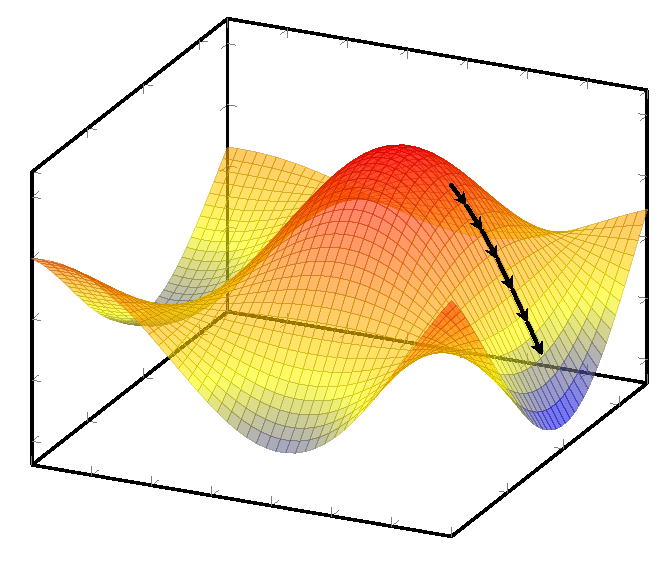
\includegraphics[scale=0.75]{tikz/chapter2 - Gradient Descent.pdf}
    \caption{Visual Representation of the Gradient Descent Algorithm}
\end{figure}

The algorithm proceeds by iteratively updating the parameters according to the gradient direction \textbf{until convergence is reached or a predefined number of iterations is completed}. By following this process, Gradient Descent effectively navigates the parameter space to find the optimal configuration that minimizes the loss function.


\subsection{The Problem of Local Minima}

In neural networks, the optimization problem is non-convex, leading to the existence of \textbf{local minima}. However, practitioners have found that these local minima are often still effective solutions. Thus, local minima are not typically a significant concern in neural network training. Below, we show an example illustrating the local minima problem for a better insight.

\begin{figure}[!htbp]
    \centering
    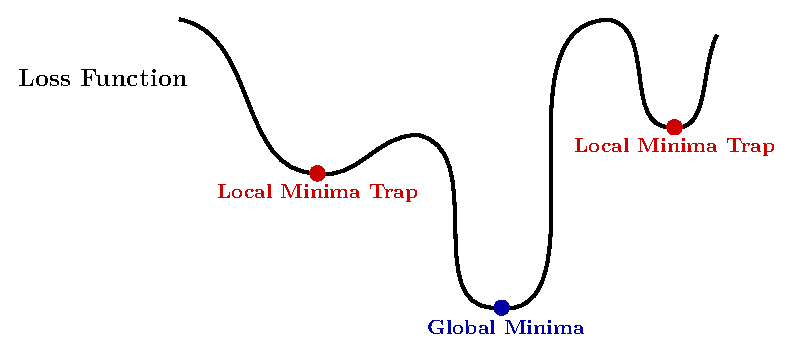
\includegraphics[scale=0.9]{tikz/chapter2 - Local Minima.pdf}
    \caption{Local and Global Minima}
\end{figure}

\subsection{The Problem of Saddle Points}

Another optimization challenge arises from saddle points, where some directions curve upwards and others downwards. At a saddle point, the \textbf{gradient is zero}, even if the point is not a minimum. saddle points are common in high-dimensional spaces. However, they only become problematic if the optimization algorithm becomes stuck exactly at the saddle point.

\begin{figure}[!htbp]
    \centering
    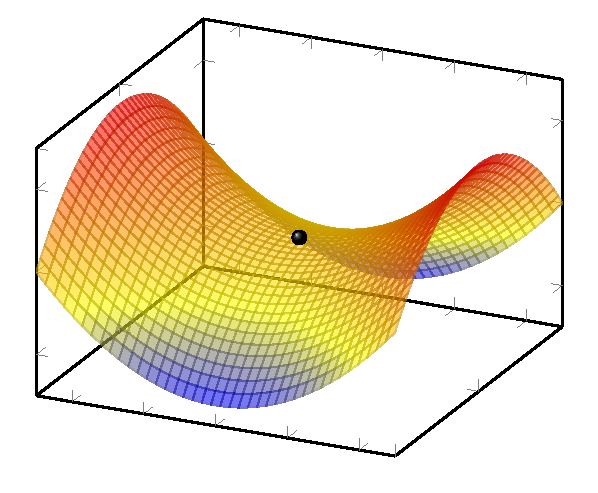
\includegraphics[scale=0.88]{tikz/chapter2 - Saddle Point.pdf}
    \caption{Saddle Point Illustration}
\end{figure}

In the figure, there is a saddle point depicted within the neural network optimization scenario, represented by the black dot. 

\section{Backpropagation Algorithm}

\subsection{Backpropagation Fundamentals}
How do we learn the weights of a neural network? Let us examine some ideas that have guided the development of learning algorithms in the context of neural networks.

The initial idea was to \textbf{randomly perturb one weight at a time}, evaluating whether that change improved model performance and saving the change. This approach, although similar to an evolutionary process, proved to be very inefficient, requiring numerous passes over the training data for each change in the weights and presenting difficulties in the last stage of learning.

Another idea involved \textbf{perturbing all the weights simultaneously} and correlating performance improvement with changes in the weights. However, this method proved equally inefficient and extremely difficult to implement.

Subsequently, a more efficient idea was proposed: to \textbf{perturb only the activations}, which are fewer in number than the weights. Although this approach is an improvement over the previous ones, it is still inefficient.

\textit{Therefore, how can we achieve more efficient learning?} This is where backpropagation comes in.

\begin{remark}{black}{white}
Backpropagation is a widely used learning algorithm in neural networks, which consists of three main steps:

\begin{enumerate}
    \item \textbf{Forward Propagation}: summation of inputs, production of activations and propagation of output through the network.

    \item \textbf{Error Estimation}: comparison of labels with predictions obtained from the network.

    \item \textbf{Backpropagation} of the error signal and using this signal to update the weights by computing gradients.
\end{enumerate}
\end{remark}

Starting from the training data, we do not directly know the optimal behavior of the hidden units within the neural network. However, using backpropagation, we can calculate how quickly the overall error of the network changes when we change the activity of these hidden units.

Using the derivatives of the error with respect to the hidden activities, we are able to understand \textbf{how each hidden unit affects the overall error of the network}. This allows us to gain a clear view of the separate effects that each hidden unit has on the error and how these effects are combined to determine the optimal direction to update the network weights.

Once we have calculated the derivatives of the error with respect to the hidden activities, we gain valuable information to update the weights associated with each connection in the network. This allows us to adjust the weights in a way that minimizes the overall error in the network, moving us closer and closer to the optimal solution for the learning problem.

\section{Exploring Backpropagation: Step by Step}

In this section, we will explore backpropagation of the error through a neural network in detail, starting with the output layer and proceeding to the input layer. We begin with a neural network composed of \textbf{one neuron per layer}.

\begin{minipage}{0.45\textwidth}
\includegraphics[width=\textwidth]{tikz/chapter2 - Chain Rule One Layer.pdf}
\captionof{figure}{Conceptualisation of Calculations}
\end{minipage}
\begin{minipage}{0.55\textwidth}
After performing the forward step, we will get an output from the last activation \( a^{(l)} \), which will allow us to calculate the loss \( \textcolor{myred}{L} \) using the desired output \( y \). The latter activation \( a^{(l)} \) is calculated using three elements: a weight \( \textcolor{myblue}{w^{(l)}} \), a bias \( \textcolor{myorange}{b^{(l)}} \), and the activation of the preceding neuron \( a^{(l-1)} \). The resulting equations are as follows:

$$ \textcolor{mygreen}{z^{(l)}} = \textcolor{myblue}{w^{(l)}} a^{(l-1)} + \textcolor{myorange}{b^{(l)}} $$
$$ a^{(l)} = \sigma(\textcolor{mygreen}{z^{(l)}}) $$
Where \textcolor{mygreen}{$z^{(l)}$} is the input of a non-linear function $\sigma$, such as a sigmoid or a ReLU. \\

A way you might conceptualize this is that the weight \( \textcolor{myblue}{w^{(l)}} \), the prior activation \( a^{(l-1)} \), and the bias \( \textcolor{myorange}{b^{(l)}} \) together \textbf{\textcolor{myyellow!85!black}{allow us to calculate}} \( \textcolor{mygreen}{z^{(l)}} \), which in turn \textbf{\textcolor{myyellow!85!black}{allow us to calculate}} \( a^{(l)} \), which together with the desired output \( y \) \textbf{\textcolor{myyellow!85!black}{allows us to calculate the loss}} \( \textcolor{myred}{L} \). This concept is illustrated in the diagram on the left.
\end{minipage}

Our initial goal during the backward step is to understand how sensitive the loss \( \textcolor{myred}{L} \) is to small changes in the weight \( \textcolor{myblue}{w^{(l)}} \), that is, calculate the derivative\( \frac{\textcolor{myred}{\partial L}}{\textcolor{myblue}{\partial w^{(l)}}} \). 
Conceptually, when you see this kind of formula, we need to think of it as saying to us "\textbf{how much does \( \textcolor{myred}{L} \) (numerator) change if we make a small change at \( \textcolor{myblue}{w^{(l)}} \) (denominator)?}"

When we calculate this derivative, we note that a small change in weight \( \textcolor{myblue}{w^{(l)}}\) \textbf{\textcolor{myyellow!85!black}{causes a change in}} \( \textcolor{mygreen}{z^{(l)}} \), which in turn \textbf{\textcolor{myyellow!85!black}{causes a change in}} \( a^{(l)} \), \textbf{\textcolor{myyellow!85!black}{directly affecting}} the loss \( \textcolor{myred}{L} \). And so this is where the chain of derivatives rule comes into play! 

As can be seen below we can now "chunk" the previous derivative:

\vspace{-0.8cm}
{\Large
% $$
\begin{equation*}
\hspace*{1cm}
\frac{\textcolor{myred}{\partial L}}{\textcolor{myblue}{\partial w^{(l)}}} = \frac{\textcolor{mygreen}{\partial z^{(l)}}}{\textcolor{myblue}{\partial \tikzmarkk{Z}w^{(l)}}}  
\frac{\partial a^{(l)}}{\textcolor{mygreen}{\partial \tikzmarkk{Y}z^{(l)}}} \frac{\textcolor{myred}{\partial L}}{\partial \tikzmarkk{YC}a^{(l)}}
\end{equation*}
% $$
\begin{tikzpicture}[overlay,remember picture]
    \node (Ze) [below of = Z, node distance = 4 em, anchor=west] {\footnotesize How much does a little variation to \( \textcolor{myblue}{w^{(l)}} \) changes \( \textcolor{mygreen}{z^{(l)}} \)?};
    \draw[<-, in=180, out=-90] (Z.south)++(.25em,-1ex) to (Ze.west);

    \node (Ye) [below of = Y, node distance = 3 em, anchor=west] {\footnotesize How much does a little variation to \( \textcolor{mygreen}{z^{(l)}} \) changes \( a^{(l)} \)?};
    \draw[<-, in=180, out=-90] (Y.south)++(.25em,-1ex) to (Ye.west);

    \node (YCe) [below of = YC, node distance = 2 em, anchor=west] {\footnotesize How much does a little variation to \( a^{(l)} \) changes \( \textcolor{myred}{L} \)?};
    \draw[<-, in=180, out=-90] (YC.south)++(.25em,-1ex) to (YCe.west);
\end{tikzpicture}
}
\vspace{1.8cm}

\textit{What about the bias term? Easy peasy!} We use the same method as for the weight term:

\vspace{-0.3cm}
$$\frac{\textcolor{myred}{\partial L}}{\textcolor{myorange}{\partial b^{(l)}}} = \frac{\textcolor{mygreen}{\partial z^{(l)}}}{\textcolor{myorange}{\partial b^{(l)}}}  \frac{\partial a^{(l)}}{\textcolor{mygreen}{\partial z^{(l)}}} \frac{\textcolor{myred}{\partial L}}{\partial a^{(l)}}$$

\textit{Now what? For the other layers?} Let's go back to our scheme for a moment and extend it:

\begin{figure}[htbp]
\centering
\includegraphics[width=\textwidth]{tikz/chapter2 - Chain Rule Multiple Layer.pdf}
\caption{Conceptualisation of Calculations (Extended)}
\end{figure}

All other weights and biases are in the earlier layers of the network, which means that their influence on cost is less direct. The way we handle them is to first consider how sensitive the cost is to the value of that activation in the penultimate layer, \( a^{(l-1)} \), and then consider how sensitive that value is to all the previous weights and biases.

The derivative of cost with respect to that activation looks a lot like what we have already seen:

\vspace{-0.5cm}
$$\frac{\textcolor{myred}{\partial L}}{\partial a^{(l-1)}} = \frac{\textcolor{mygreen}{\partial z^{(l)}}}{\partial a^{(l-1)}}  \frac{\partial a^{(l)}}{\textcolor{mygreen}{\partial z^{(l)}}} \frac{\textcolor{myred}{\partial L}}{\partial a^{(l)}}$$

The trick here is to remember that the activation in the previous layer is determined by its set of weights and biases. For example, there is a long chain of dependencies between the weight \( w^{(l-1)} \) and the cost \( \textcolor{myred}{L} \). The way this presents itself mathematically is that the partial derivative of the cost with respect to that weight appears as a long chain of partial derivatives for each intermediate step, see the image below to visualize the concept graphically.

\begin{minipage}{0.55\textwidth}

Here is how you can decompose the derivative:

\vspace{-0.3cm}
$$\frac{\textcolor{myred}{\partial L}}{\textcolor{myblue}{\partial w^{(l-1)}}} = 
\frac{\textcolor{mygreen}{\partial z^{(l-1)}}}{\textcolor{myblue}{\partial w^{(l-1)}}}  
\frac{\partial a^{(l-1)}}{\textcolor{mygreen}{\partial z^{(l-1)}}} 
\underbrace{
\frac{\textcolor{mygreen}{\partial z^{(l)}}}{\partial a^{(l-1)}}  
\frac{\partial a^{(l)}}{\textcolor{mygreen}{\partial z^{(l)}}} 
\frac{\textcolor{myred}{\partial L}}{\partial a^{(l)}}}_\textrm{\Large$\frac{\textcolor{myred}{\partial L}}{\partial a^{(l-1)}}$}$$
\vspace{-0.3cm}
\ \\
By following the dependencies through our tree and multiplying together a long series of partial derivatives, we now \textbf{can calculate the derivative of the cost with respect to any weight or bias of the entire network}. \textit{We are simply applying the same idea of the chain rule that we have always used!} \\

And since we can get any derivative, we can calculate the entire gradient vector:
\vspace{-0.1cm}
$$
\Delta_w L = \left[ \frac{\textcolor{myred}{\partial L}}{\textcolor{myblue}{\partial w^{(1)}}}, \frac{\textcolor{myred}{\partial L}}{\textcolor{myorange}{\partial b^{(1)}}}, \ldots , \frac{\textcolor{myred}{\partial L}}{\textcolor{myblue}{\partial w^{(l)}}}, \frac{\textcolor{myred}{\partial L}}{\textcolor{myorange}{\partial b^{(l)}}}\right] 
$$
\vspace{-0.3cm}
\ \\
The job is done! At least for this network, now we must add more neurons for each layer. \textit{I know, you are crying inside, but actually, not much changes when we give the layers more neurons: it's just a few more indexes to keep track of \emoji{smile}}.

\vspace{1cm}

\end{minipage}
\begin{minipage}{0.45\textwidth}
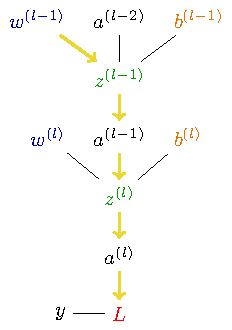
\includegraphics[width=\textwidth]{tikz/chapter2 - Chain Rule Multiple Layer Dependencies.pdf}
\captionof{figure}{Calculations with 3 Layers}
\end{minipage}

\begin{minipage}{0.4\textwidth}
\includegraphics[width=\textwidth]{tikz/chapter2 - Indexing.pdf}
\captionof{figure}{Neural Network Indexing}
\vspace{0.8cm}
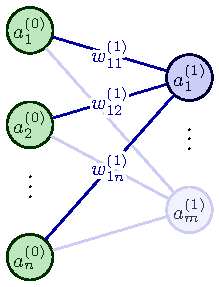
\includegraphics[width=\textwidth]{tikz/chapter2 - Indexing Example.pdf}
\captionof{figure}{Example of Indexing}
\end{minipage}
\begin{minipage}{0.05\textwidth}
\
\end{minipage}
\begin{minipage}{0.55\textwidth}
When dealing with neural networks with multiple neurons per layer, we have to change the notations a bit.\\

The activation of each neuron will be denoted with a subscript indicating its position within the layer. Thus, \textbf{the superscript of each neuron indicates which layer it is in, while the subscript indicates the specific neuron}.\\

The weights also need a refresh: additional indices are required to specify their location. In addition to the superscript representing the layer, \textbf{two subscripts indicate the edge weight connecting the neuron in layer $i$ to the neuron in layer $j$}.\\

\textit{I know, these "$ji$" indices, being backwards, might seem strange or unconventional at first, but they align with the way the weight matrix is usually indexed.}\\

On the left are two images: one formally represents how the nodes and edges of the network are represented, while the other provides an example with two dummy layers, named $0$ and $1$, with $n$ and $m$ nodes, respectively.
\end{minipage}

\newpage
The weighted sum \textcolor{mygreen}{$z_{j}^{(l)}$} then takes the following form:
$$
\textcolor{mygreen}{z_{j}^{(l)}} = \sum_{i} \textcolor{myblue}{w_{ji}^{(l)}} a_i^{(l-1)} + \textcolor{myorange}{b_{j}^{(l)}}
$$
The new equations turn out to be esentially the same with respect to the case of only one neuron per layer:

\vspace{-0.4cm}
$$
\frac{\textcolor{myred}{\partial L}}{\textcolor{myblue}{\partial w_{ji}^{(l)}}} = \frac{\textcolor{mygreen}{\partial z_{j}^{(l)}}}{\textcolor{myblue}{\partial w_{ji}^{(l)}}}  
\frac{\partial a_{j}^{(l)}}{\textcolor{mygreen}{\partial z_{j}^{(l)}}} \frac{\textcolor{myred}{\partial L}}{\partial a_{j}^{(l)}}
$$

Indeed, the expression of the derivative of the chain rule describing the sensitivity of cost with respect to a particular weight is the same as in the previous case. The only difference is that we now have multiple indices, $i$ and $j$, indicating which weight we are considering.

What changes, however, is the derivative of the cost with respect to one of the activations in the preceding layers, because \textbf{the preceding neurons influence the cost function through multiple pathways}.

To understand the sensitivity of the cost function with respect to a certain neuron, it is necessary to sum the influences along each of these different pathways. So, we \textbf{sum multiple expressions of different chain rules corresponding to each pathway of influence}.

\vspace{-0.5cm}
$$\frac{\textcolor{myred}{\partial L}}{\partial a_{i}^{(l-1)}} = \underbrace{\sum_{j}\frac{\textcolor{mygreen}{\partial z_{j}^{(l)}}}{\partial a_{i}^{(l-1)}}  \frac{\partial a_{j}^{(l)}}{\textcolor{mygreen}{\partial z_{j}^{(l)}}} \frac{\textcolor{myred}{\partial L}}{\partial a_{j}^{(l)}}}_\textrm{Sum over layer $l$}$$

This reasoning is carried out using traditional numerical values, but it is evident that in order to efficiently handle the weights and biases of the neural network, it is necessary to use the \textbf{matrix approach}, since it allows simultaneous operations to be performed on all the parameters of the network, greatly optimizing the computational process.
